\chapter{Background \& Related Work}

\section{Background}

% \subsection{Lead Sheets}

% Lead sheets are a form of musical notation that contain both the melody and harmony. Only the dominant melody is present which is often the vocal line and is written in standard musical notation on a stave. The harmony is represented by chord symbols, which are written above the stave at the relevant time. A lead sheet also contains the key, time signature and, optionally, the lyrics of a song. An example of a lead sheet is shown in Figure~\ref{fig:lead_sheet_example}.

TODO:
Rewrite background to focus on background chord recognition.

- Chords, harmony, ambiguity and importance
- Chord recognition as a subfield of music transcription and older related papers.
- Connection to lead sheets, definition.

\begin{figure}[h]
    \centering
    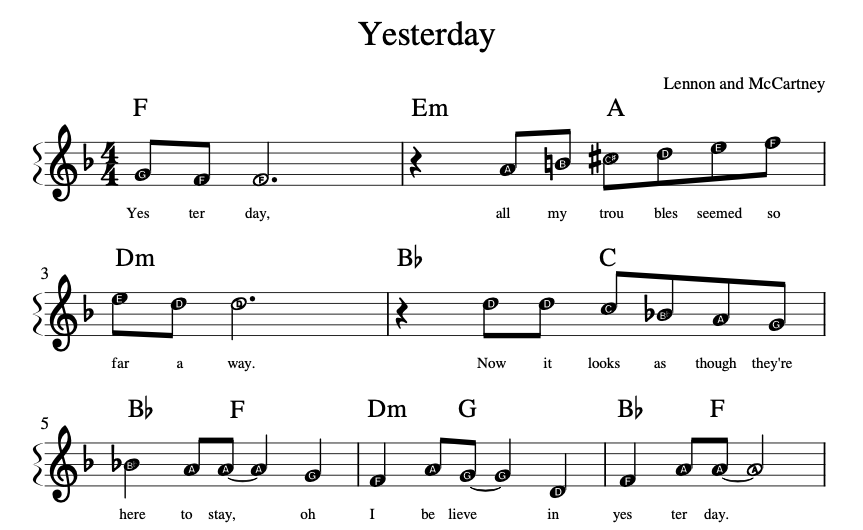
\includegraphics[width=0.8\textwidth]{figures/lead_sheet_example.png}
    \caption{An example of a lead sheet for `Yesterday' by the Beatles.}
    \label{fig:lead_sheet_example}
\end{figure}

% Lead sheets are most notably used in jazz music where their origins lie. They date back to the mid 20th century, and were originally called `fake sheets' because they were used by musicians to `fake' their way through a song~\citep{RealBookPodcast}. Any jazz musician worth their salt owns a `real book', so called to distinguish it from the fake books that were used in the past. Real books contain lead sheets for hundreds of jazz standards, and are still an essential tool for any seasoned jazz musician. 

% More recently they have served as a useful tool for musicians in other genres too, such as pop and rock, who want to learn and perform songs quickly and easily. They allow efficient communication of the important elements of a song, without the need for a full score, encouraging further improvisation and personalisation of the song.

% Lead sheets do not contain all the information of a full score, such as dynamics, articulation, or specific voicings of chords. Furthermore, they are not suitable for all types of music, such as classical music, where a full score is necessary to convey the composer's intentions, or rap music where the lyrics and beat are normally the most important elements. However, they are a useful tool for many musicians, and are a common way of representing music for both learning and performing.

% \subsection{Automatic Music Transcription}

% Automatic Music Transcription (AMT) is a field within Music Information Retrieval (MIR) that aims to construct models that convert musical audio into symbolic representations.~\citep{ComprehensiveReviewMusicTranscription} provide a comprehensive review of different forms of transcription. For lead sheet transcription, we are interested in their highest level of transcription: notation-level. We want to be able to take an audio recording of a song and generate a lead sheet that contains the melody and harmony of the song. This is a challenging task, as it requires the model to isolate and transcribe a melody, transcribe the chordal information, and then combine these two elements into a coherent lead sheet where the melody and harmony are aligned in time/beat.

% There are three sub-fields of musical transcription that are of interest to lead sheet generation: Automatic Chord Recognition (ACR), Melody Transcription (previously called F0 estimation) and Beat Detection.


\subsection{Music Features}\label{sec:background-features}

Recorded music can be represented in a variety of ways as input to a machine learning model. The simplest way is to leave the data as a waveform: a time-series vector of amplitudes. Data in the raw audio domain has seen successful use in generative models such as Jukebox~\citep{Jukebox} and RAVE~\citep{RAVE}.

A very commonly used representation of general audio data, and specifically musical data, is the spectrogram. A spectrogram is a conversion of the time-series data into the time-frequency domain, calculated by a SFTF (short-time Fourier Transform) Spectrograms are commonly used in many audio processing tasks, such as speech recognition, music recognition~\citep{ShazamSpectrogram} and music transcription, specifically polyphonic transcription~\citep{PianoTranscriptionWithTransformer}. However, as noted by~\citet{20YearsofACR}, only logarithmic spectrograms have been used in ACR tasks, and linear spectrograms have been used in melody transcription tasks.

A common version of the spectrogram used in music transcription is the Constant-Q Transform (CQT), originally proposed by~\citet{CQT}. The CQT is a version of a spectrogram with frequency bins that are logarithmically spaced and bin widths that are proportional to the frequency. This is motivated by the logarithmic nature of how humans perceive pitch: a sine wave that is perceived as one octave higher than another has double the frequency. The CQT is used in many music transcription tasks, such as automatic chord recognition~\citep{FirstDeepLearningCQT}, and a popular alternative, Melspectrograms, have found use in melody transcription~\citep{PianoTranscriptionWithTransformer}. An example CQT from the dataset used in this work is shown in Figure~\ref{fig:cqt_example}.

\begin{figure}[h]
    \centering
    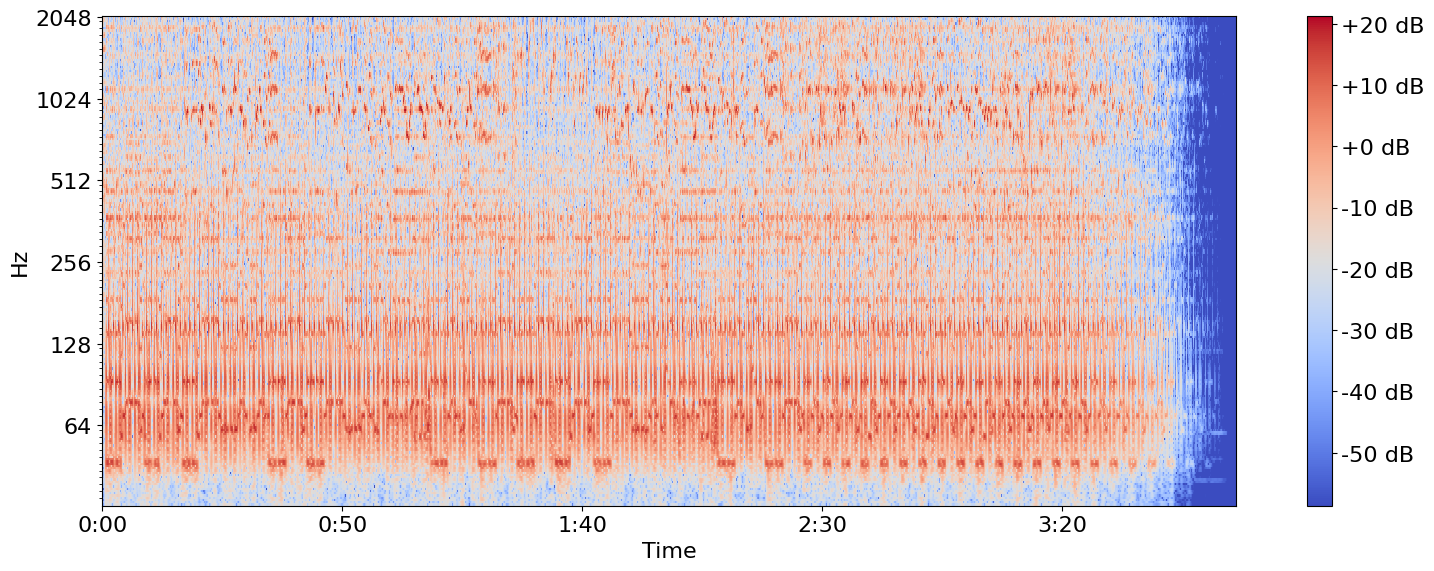
\includegraphics[width=1\textwidth]{figures/sample_cqt.png}
    \caption{A sample CQT of `Girls Just Wanna Have Fun' by Cyndi Lauper from the dataset used in this work. We can clearly see the log-spaced frequency bins. We also observe clear structure and repetition in the song, espeically in the lower frequencies, which can be attributed to a regular drum groove and bass instruments. This is typical of pop songs in this dataset.}~\label{fig:cqt_example}
\end{figure}

Chroma vectors are a 12-dimensional time-series representation, where each dimension corresponds to a pitch class. Each element represents the presence of each pitch class in the Western chromatic scale in a given time frame. Such features have been generated by deep learning methods~\citep{BalanceRandomForestACR} or by hand-crafted methods~\citep{NNLSChroma} and have seen use in recent ACR models~\citep{HarmonyTransformer}.

More recently, features extracted generative models have been used as input. The proposed benefit is that the vast quantities of data used to train these models allows for rich representations of the music.~\citet{MelodyTranscriptionViaGenerativePreTraining} use features from JukeBox~\citep{Jukebox} to train a transformer~\citep{AttentionIsAllYouNeed} for both melody transcription and chord recognition and combine these into a lead sheet generation model. They found that these features outperformed hand-crafted features in melody transcription tasks but did not perform experiments in ACR.

\section{Related Work}

\subsection{Automatic Chord Recognition}\label{sec:background-acr}

\cite{20YearsofACR} provides an overview of ACR since its inception in 1999 with the work of~\citet{FujishimaACR} up to 2019, and provide suggestions for future avenues of research. Among them are the lack of exploration of feature and chord representations and the imbalance with chords classes present in chord datasets.

Datasets that have seen common use in ACR relevant to this work include:
\begin{itemize}
    \item \emph{Mcgill Billboard}: 890 chord annotations of songs randomly selected from the Billboard `Hot 100' Chart bnetween 1958 anmd 1991.~\citep{McgillBillboard}
    \item \emph{Isophonics}: 300 annotations of songs from albums by The Beatles, Carole King and Zweieck.~\citep{Isophonics}
    \item \emph{RWC-Pop}: 100 pop songs with annotations available\footnote{\url{https://github.com/tmc323/Chord-Annotations}} for chords.~\citep{RWC}
    \item \emph{USPop}: 195 annotations of a larger dataset with artists chosen for popularity.~\citep{USPop}
    \item \emph{JAAH}: 113 annotations of a collection of jazz recordings.~\cite{JAAH}
    \item \emph{HookTheory}: 50 hours of labelled audio in the form of short musical segments, crowdsourced from the HookTheory website\footnote{https://www.hooktheory.com/}.~\citep{MelodyTranscriptionViaGenerativePreTraining}
\end{itemize}

Other small datasets also exist. Many of these have been compiled together into the \emph{Chord Corpus} by \citet{Choco}, with standardised annotation formats.

A variety of machine learning methods have been applied to such datasets. Older methods such as ~\cite{ACRHMM} use HMMs, but more recent methods use deep learning. Often, CNNs and RNNs are used in combination~\citep{ACRCNNRNN1,ACRLargeVocab1,StructuredTraining} with CNNs performing feature extraction from a spectrogram feature, and an RNN (normally Bi-LSTM or Bi-GRU) predicts chord sequences. More recently, transformers have been applied to the entire process~\citet{MelodyTranscriptionViaGenerativePreTraining} and~\citet{HarmonyTransformer,AttendToChords}.

Evaluation is typically done using accuracy and recall of correct chord predictions, or more music-aware measures such as the correct root note, 3rd or the MIREX metric which measures that chords have at least 3 notes in common. These are all implemented by \citet{MIREVAL} in the \texttt{mir\_eval} library~\footnote{\url{https://mir-evaluation.github.io/mir_eval/}}. Qualitative evaluation is also often carried out.

A big problem frequently encountered in ACR is the lack of labelled data. This work uses 1200 labelled songs with audio. This is due to the difficulty and time associated with labelling data aligned in time and the legal sensitivity of the data involved.Data has been scaled up using augmentation and semi-supervised learning~\citep{ScalingUpSemiSupervisedLearning} with some success. Research has been done into the use of synthetic data~\citep{MusicGenTrainingData,AnnotationFreeSyntheticData} and supervised learning~\citep{MERTSupervisedLearning} for MIR tasks, but not for ACR.

Another problem is that the existing data is often imbalanced, with a large number of common chords like major and minor chords and fewer chords like diminished and augmented chords, or chords with upper extensions and inversions. This can lead to models that are biased towards predicting major and minor chords. Attempts to address this have been made by re-weighting classes~\citep{ACRLargeVocab1} or adjusting the sampling of training examples to balance chord classes~\citep{BalanceRandomForestACR}.

\subsection{Lead Sheet Transcription}

Older work has attempted to automatically produce lead sheets~\citep{LeadSheet2008,LeadSheet2009}. They use hand-crafted feature extractions and probabilistic models for melody and chord classification. AMT has developed dramatically since this work which leaves much room for improvement.

\citep{MelodyTranscriptionViaGenerativePreTraining} is the only recent work we found that produces a full lead sheet generation model. They propose the use of features extracted from middle layers if Jukebox~\citep{Jukebox} which were found to lead to the best performance in downstream tasks~\citep{JukeBoxFeatureExtraction}. These features are used to train a transformer, with a primary focus on melody transcription. The model and code is available\footnote{\url{https://github.com/chrisdonahue/sheetsage/tree/main}}. They use the same methodology to train an ACR model, and combine these with beat detection and engraving software to produce a lead sheet.

The authors found the use of these generative pre-trained features to be beneficial for melody transcription. However, they use community-submitted annotations from an online forum, presumably for lack of a better alternative, whose quality and variety may be lacking. The nature of this data means that the model is only trained on 24 second audio clips, which limits performance on longer segments of audio. The authors claim that the overall model performs well, especially in the verses and choruses of pop music where vocal lines are loud and clear, and that performance across genres is surprisingly good given the pop-centric dataset. However, further analysis is ommitted and if the dataset contains music with few songs with more complex harmonic structures such as jazz music, then the model will produce overly simplistic representations of the chords. Crucially, the work does not explore ACR models beyond simply copying their method and dataset used in melody transcription and there is no quantitative evaluation of performance in ACR. Furthermore, the system can struggle with melody lines shifting between instruments, quiet vocal lines